

\section{Introduction}

\begin{example}
\textbf{Immunotherapy}. We are working on a new medical treatment and we would like to predict for each patient whether the treatment will work for her or not.
Available to us is a data set which is shown in the figure below. On the basis of this data we need a no/yes (0 or 1) prediction in order to decide whether or not to apply the treatment.
\begin{figure}[h!]
  \centering
    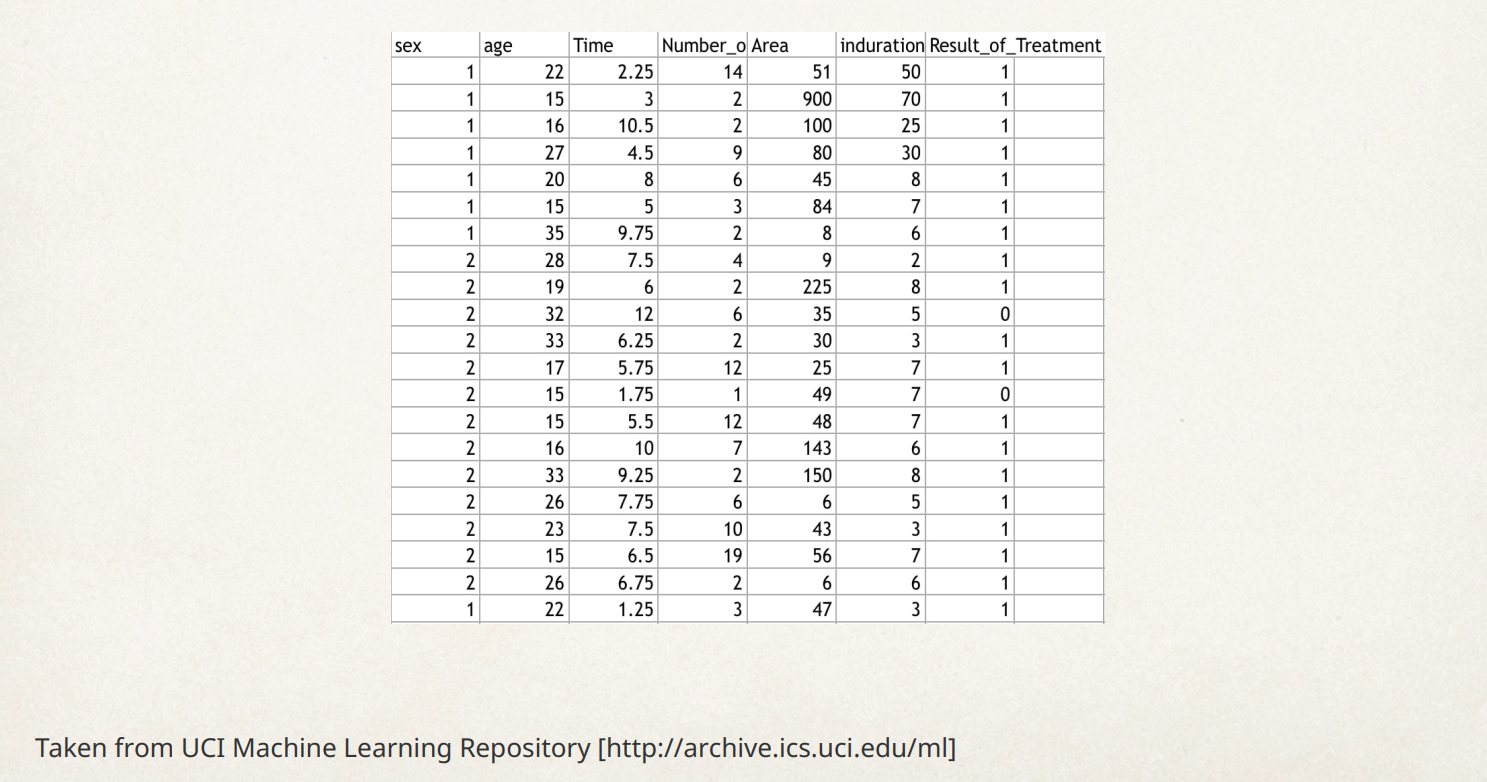
\includegraphics[scale=0.3]{chapters/pac/figures/ImmunotherapyDataSet.png}
    \caption{Immunotherapy Data Set}
\end{figure}
\end{example}

Let us list the ingredients of a general problem of this type:

\begin{itemize}
 \item The individual object, $\mathbf{x}$, that we wish to label. In our case, each such object is a vector $\mathbf{x}$ of $d$ real numbers describing $d$ features of a patient, as shown in the figure.
 \item The set of all possible $\mathbf{x}$'s is called the \textit{\textbf{Domain set, $\Xc$}}. We can take, for example,  $\Xc= \mathbb{R}^d$ (We could also take a smaller $\Xc$ since age must be positive and sex can have only two values).
 \item \textit{\textbf{Label set, $\Yc$}}: set of possible labels. In our case we can take, for example,  $\Yc=\{0,1\}$, where $0$ corresponds to a recommendation for not giving the treatment and 1 for giving it.
 \item \textbf{A prediction rule, $h:\Xc\to \Yc$}: used to label future examples. This function is called a \textbf{predictor}, a \textbf{hypothesis}, or a  \textbf{classifier}.
\end{itemize}


So the learner's input (e.g., the data in the figure) is called \textbf{Training data,} and consisting of $m$ already-labelled objects {$S=((\mathbf{x}_1,y_1),...,(\mathbf{x}_m,y_m)) \in  (\Xc\times \Yc)^m$, and the learner's output is the prediction rule, $h:\Xc\to \Yc$. So a learner is a map $\mathcal{A}:S\mapsto h$. The goal of the learner is to produce an $h$ that will be correct (as much as possible) on future examples.  So we need to have a way to quantify this, namely, to measure the quality of prediction of a candidate rule  $h$ with respect to future examples. 

\section{A Theoretical framework for learning}

The most basic questions in machine learning are: Is anything learnable? what
can be learned and what cannot? When learning is possible, how many training
samples do we need to learn? When learning is possible, how do we learn? In this lecture we develop the {\bf PAC theory of
learning}, a famous theory that gives (within its assumptions and framework) a complete
answer to this question - for {\bf batch  supervised learning}. 

\subsection{A Data-generation Model }
To formal mathematical answers to such questions, we must make formal
mathematical assumptions on how our training and test samples are generated.
From now on, we assume the following:
\begin{itemize}
  \item There is a distribution $\Dc$ over the examples $\Xc$.  That is, each $\mathbf{x}_i$ is sampled according to $\Dc$ and therefore each sequence $S$, of $m$ $\mathbf{x}$'s, has a different probability to appear.
  \item The $\mathbf{x}$'s are \textbf{Independently Identically Distributed (i.i.d.)}.
  In particular, the training set $S$ consists of $(x_i,f(x_i))_{i=1.. m}$, where the $\mathbf{x}_i$'s were sampled independently according to $\Dc$, and our test set, will be made of future examples: $x\in\Xc$, again to be  sampled according to $\Dc$ independently of each other and of those in the training set.
  \item There is a function $f$ which is the correct classifier, i.e., for every $i \in [m]$, $y_i = f(x_i)$
  For now, we assume that $f$ is deterministic (no noise): $y=f(x)$ and we will call it the "PAC model". 
  In following lectures we'll add noise and call it the "Agnostic PAC model".
\end{itemize}

Compare the above to first learning problem we saw - the Linear Model: There, we had samples\footnote{the sample space there was $\Xc=\mathbb{R}^d$} $\mathbf{x}_1,..,\mathbf{x}_m\in\mathbb{R}^d$  fixed (given) and all of them received equal importance, for example, in their contribution to the global error (the loss function). In the framework we are developing now, the samples $\{x_i\}$ are  i.i.d samples according to $\Dc$, i.e., they have different probabilities to appear and therefore may have a different weights in the loss function.
In the previous lecture we started with assumption $y_i=f(\mathbf{x}_i)$ where $f$ is deterministic and linear. We then assumed \textit{noise} $y_i = f(x_i)+z_i$. Next lecture we will add noise also to our current model.

\subsection{Classifiers}

We will focus on focus on \textbf{classifiers} until further notice. However, many principles you'll see today are true for regression problems as well.

For a classifier, we define the \textbf{Generalization Error} as:
\[
L_{\Dc,f}(h) ~\equiv~ \mathbb{P}rob_{x \sim \Dc}[h(x) \neq f(x)] ~\equiv ~ \Dc\left( \{ x \in \Xc : h(x)
  \neq f(x) \}\right) ~.
\]
where $\Dc$ and $f$ are unknowns. The generalization error is also called the \textbf{risk}, or the \textbf{true error}. Recall that $\Dc$ is a distribution over $\Xc$, that is, for a given $A \subset \Xc$, the value of $\Dc(A)$ is the probability to see some $x \in A$.

{\bf Note:} Recall that you should be critical about an error measure that counts
total number of misclassification error of a classifier. Recall that  there are two kinds of errors a classifier can make. they are called Type-I and Type-II errors and one is usually much worse than the other\footnote{For now, we only note that, assuming $\Yc =\{0,1\}$, in the above definition of the true error, $h(x) \neq f(x)$ may refer either to  $h(x)=1, f(x)=0$ or to $h(x)=0, f(x)=1$. According context of the actual learning problem at hand, one of these two cases  will correspond to a \textbf{False Positive} event and the other to a \textbf{False negative} event}.

\subsection{The framework so far} \label{sec:frame}

Make sure you understand the theoretical framework we have developed so far. Our task is to design a learning algorithm (a "learner"), which we denote by $\mathcal{A}$. For a given sample size $m$, $\mathcal{A}$  is a map from the training sample 
\[S=((x_1,y_1),..,(x_m,y_m)) \in (\Xc\times \Yc)^m\]
where each $\mathbf{x}_i$
to the set of all possible rules $\mathcal{X}\to\mathcal{Y}$. 

We're thinking of classification problems now, so in this lecture $\mathcal{Y}=\{\pm 1\}$, but everything here can be generalized. The {\bf data generation model} we assume is probabilistic, in fact i.i.d: We assume that there is an unknown distribution $\mathcal{D}$ over $\mathcal{X}$ (so that $(\mathcal{X},\mathcal{D}$) is a probability space - we won't pay attention to sigma-algebras, measurable sets and all that jazz). We assume that each sample - both in training set and it test set - is sampled according to $\mathcal{D}$ independently from any other sample before of after it. For the labels $y$, we assume there is an unknown function $f:\mathcal{X}\to\mathcal{Y}$ such that for each sample $x\in\mathcal{X}$, the corresponding label is $y=f(x)$.
In particular, for our training data, we have $y_i = f(x_i)$ for $i=1,\ldots,m$. Finally, for a candidate prediction rule $h:\mathcal{X}\to\mathcal{Y}$ that our learner may produce,  will measure the generalization performance of $h$ - how well it will perform on future unseen samples - by simply using the expected misclassification rate 
$$
L_{\Dc,f}(h) ~\equiv ~ \mathbb{P}_{x \sim \Dc}[h(x) \neq f(x)] \,.
$$

\subsection{Our goal in this lecture}

Our goal in this lecture will be to understand, in detail, the following two definitions.

\paragraph{Definition: PAC learnability and sample complexity}
\begin{enumerate}
\item
A hypothesis class $\Hc$ is {\bf PAC Learnable} if there exists a function $\tilde{m}_\Hc : (0,1)^2 \to \N$ and a learning algorithm $\Ac$ with the following property:
For every $\epsilon,\delta \in (0,1)$ and for every distribution $\Dc$ over $\Xc$, and for every labeling function $f:\Xc\to\{\pm 1\}$ that satisfies $L_{\Dc,f}(h^*)=0$ for some $h^*\in\Hc$, when running the learning algorithm $\Ac$ on $m\ge \tilde{m}_\Hc(\epsilon,\delta)$ i.i.d. examples generated by $\Dc$ and labeled by $f$, the algorithm returns an hypothesis $h_S=\Ac(S)$ such that, with probability of at least $1-\delta$ (over the choice of the training samples), we have
$
L_{\Dc, f}(h_S) \le \epsilon
$. 
\item For a PAC learnable hypothesis class, we define the {\bf Sample
  Complexity} of $\Hc$ for specified $\epsilon,\delta$ as the minimal number of
  samples $\tilde{m}_\Hc(\epsilon,\delta)$ required for the definition to hold
  with respect to $\epsilon,\delta$. The Sample Complexity function of $\Hc$ is
  denoted $m_\Hc:(0,1)^2\to\mathbb{N}$.
\end{enumerate}

\paragraph{Definition: VC-Dimension}
~\\Let $\Hc\subset\left\{ \pm 1 \right\}^\Hc$ be an hypothesis class.
For a subset $C\subset \Xc$ let $\Hc_C$ be the restriction of $\Hc$ to $C$, namely,
$\Hc_C = \{ h_C : h \in \Hc\}$, where for $h:\Xc\to\Yc$, $h_C:C\to\Yc$ is the
function such that $h_C(x)=h(x)$ for every $x\in C$. Define the {\bf VC-dimension} of $\Hc$ by
\[
  VCdim(\Hc) := \max\{ |C| ~\Big|~ C\subset\Xc \,\,\text{and}\,\, |\Hc_C|=2^{|C|} \}
  \,.
\]
\\~\\
Note that $VCdim(\Hc)\leq \infty$. 

\paragraph{The Fundamental Theorem of Statistical Learning.}
~\\
These two definitions are interesting since, if we adopt PAC learnability as our
notion of learnability, then we have a {\bf complete characterization of when it
is possible (and impossible) to learn, in terms of the VC-dimension, as well as  the exact minimal  training sample size we need in order to learn, and a "universal" learner that successfully learns when enough training data is available. } In short, we have a full theory of batch learning - a full theory of when it is possible to generalize from a training sample to new samples, and how to do it.
\\~\\
This result is sometimes known as ``the fundamental theorem of statistical
learning'' and states the following (roughly):
\begin{itemize}
  \item An hypothesis class $\Hc$ is PAC-learnable {\bf if and only} if
    $VCdim(\Hc)<infty$
  \item The sample complexity of an hypothesis class with finite VC-dimension is
    roughly\[
m_H(\epsilon,\delta) \sim \frac{VCdim(\Hc)+\log(1/\delta)}{\epsilon}
\]
\item The ERM rule achieves this minimum, namely, when learning is possible, ERM
  learns with a minimial number of examples.
\end{itemize}

Since the definitions of PAC-learnability and VC-dimension are quite complicated, we will take the rest of the lecture to slowly unpack them. So now, let's put ourselves in the framework as it appears in Section \ref{sec:frame}, and advance from there in baby steps. 

\subsection{Learning as a Game - first attempt}

This framework in Section \ref{sec:frame} can be thought of as a {\bf game} between us and Nature, with a random payoff. The game proceeds as follows. The number of training samples $m$ is given in advanced as a game parameter. \\

We move first. We choose a learner $\mathcal{A}$ that trains on $m$ samples. This is our strategy.
Nature moves second. Nature chooses a distribution $\mathcal{D}$ and a labeling function $f$. This is Nature's strategy. Importantly, Nature knows the strategy we chose when she chooses her strategy.
To calculate the game's payoff, an i.i.d sample $S$ of length $m$ is drawn according to the distribution $\mathcal{D}$ that Nature chose, is labeled according to the function $f$ that Nature chose, and is fed into the learner $\mathcal{A}$ that we chose to obtain the prediction rule $h_S:=\mathcal{A}(S)$ (the notation $h_S$ helps us remember that the prediction rule we learn, $h_S$, strongly depends on the random sample $S$ that we drew). The payoff is $L_{\Dc,f}(h)$. We can think that we want it to be as small as possible, and maybe Nature is an adversary that wants it to be as large as possible. Note that the payoff is random as it depends on the sample $S$ that was drawn. If we're unlucky, and the sample $S$ is "bad", namely, does not represent $\mathcal{D}$ very well, then the rule $h_S$ our learner produces might not generalize well and the random loss (for that draw of $S$) will be high. 

Now you might ask: what's the best strategy for us (how to best design $\mathcal{A}$)? 
Remember that Nature will know what we chose, and can try to be "cruel", namely, to choose $\Dc$ and $f$ that our learner did not prepare well for. Also, there's always a chance that we will draw a "lousy" sample $S$, namely a misleading sample that will confuse our learner and will cause it to output a rule $h_S$ that will not generalize well. Is there a way to "defend" ourselves against "cruel" strategies $\mathcal{D},f$ that Nature might play, and against "unlucky" draws of a training sample $S$? Is there anything at all that can be said in this generality about the problem of learning (= the problem of generalizing from training samples to new samples)? 

~\\
Let's define this as {\bf The Learning Game (first version)}:
Fix the sample size $m$. Let's view our framework as a game between us and
  Nature, with random payoff.
  \begin{itemize}
  
    \item We choose a strategy (namely, a learner) $\Ac:(\Xc,\Yc)^m \to \Yc^\Xc$
      \item Nature knows our strategy, and, after us, chooses strategy that consists of a probability distribution $\Dc$ over $\Xc$, and a label function $f:\Xc\to\Yc$. 
    \item A sample $S$ of size $m$ is drawn according to $\Dc$ and is labeled
      according to $f$
    \item The sample $S$ is fed into $\Ac$ to produce a prediction rule
      $h_S=\Ac(S)$
    \item The payoff is $L_{\Dc,f}(h_S)$, namely, the expected fraction of misclassification errors $h_S$ will make on data drawn i.i.d according to $\Dc$ and labeled according to $f$.
    {\bf The payoff is random since $S$ is random and
      therefore $h_S$ is random.}
    \item We are going to assume Nature is ``cruel'' and does her best to win.
      So we'll look for learners $\Ac$ that have a {\bf guaranteed maximal 
      loss} $L_{\Dc,f}(h)$ {\bf for any} strategy $\Dc,f$ that Nature might play.
\end{itemize}
